\chapter{Diseño e implementación}
\label{cap:Diseno}

El presente capítulo detalla la fase de diseño y construcción de la aplicación, se señalan las decisiones tomadas a lo largo del desarrollo para cumplir con los requerimientos presentados en capítulo anterior.

Desde lo general a lo particular, se comienza presentando la arquitectura del sistema, construida a partir de los requerimientos establecidos en el capítulo anterior. Posteriormente se analizan las decisiones que llevaron al diseño de dicha arquitectura.

\section{Arquitectura del sistema}
\label{sec:Arquitectura}

El sistema de detección de necesidades, en su conjunto, consta de dos módulos independientes: el \textit{front-end}, dedicado a la interacción con el usuario, presentación de la información, etcétera; y el \textit{back-end}, orientado a las tareas de procesamiento \textit{online} de los datos para su posterior despliegue.

La comunicación entre los módulos se realiza por medio del almacenamiento de documentos en la base de datos. Esta arquitectura se presenta en la Figura \ref{fig:arquitecturaSistema}. A continuación se detalla cada uno de los elementos que la componen.

\begin{figure}[H]
	\centering
	\captionsetup{justification=centering}
	\includegraphics[scale=0.6]{images/arquitectura.png}
	\caption[Arquitectura del sistema.]{Arquitectura del sistema.\\Fuente: Elaboración Propia, (2016)}
	\label{fig:arquitecturaSistema}
\end{figure}

\subsection{\textit{Back-end}}
\label{subsec:backend}

El módulo de \textit{back-end} corresponde al sistema de detección en sí, todo el sistema está alimentado por el \textit{stream} entregado por la API de \textit{Twitter}, pues en esta red social se generan más de 140 millones de \textit{tweets} diariamente y que se incrementa en períodos de crisis, \cite{TaxonomiaChato}, \cite{StormIBM}, por ello es considerada una fuente de información primaria, es decir, aquella que viene directamente de la población afectada. Haciendo uso de esta fuente de información se da soporte a la historia de usuario HU-c02, que explicita su uso.

Para el procesamiento de los datos que llegan de forma continua se hace uso de \textit{Apache Storm} para construir un grafo de procesamiento \textit{ad-hoc} a la aplicación, capaz de detectar y categorizar todos aquellos eventos que respondan a los requerimientos de la aplicación. Para ello se utilizan los elementos de \textit{Storm} presentados en la sección \ref{arte:SPS}, \textit{spout} y \textit{bolt} para la construcción de operadores que realicen las tareas necesarias para la transformación de datos. Uno de estos operadores tiene que ver con cómo son compartidos los datos, en este caso, se hace uso de una base de datos no relacional, MongoDB, para compartir datos entre módulos y permitir una comunicación bidireccional, tanto de consultas como de elementos a ser desplegados en la visualización. Otro de los operadores tiene que ver con el etiquetado de datos, para ello se hace uso de un clasificador, almacenado como un un archivo. Este operador es generado haciendo uso de Mallet para etiquetar las nuevas entradas como elementos de una categoría en particular. El cómo funcionan estos operadores se detalla a lo largo de este capítulo.

Los elementos cuya comunicación se señala con una flecha roja son elementos que están considerados en la arquitectura final, pero que están fuera de los alcances de del proyecto, ellos son el sistema detector de eventos que, al detectar que se produce un evento catastrófico en el país, comienza a ejecutar el detector de necesidades y el módulo etiquetador que recibe un archivo con entradas con eventos etiquetados, los cuales puede utilizarse para reentrenar el clasificador con el objetivo de mejorar su capacidad de clasificación.

\subsection{\textit{Front-end}}
\label{subsec:front}

El módulo correspondiente a la visualización está encargado de desplegar la interfaz de usuario al sistema por medio de su navegador \textit{Web}. El módulo hace uso de la información registrada por el módulo de detección de necesidades, la cual es almacenada en la base de datos para mostrarla al usuario. 

Para cumplir con las funcionalidad requeridas se utilizó la API de Google Maps para implementar una instancia de mapa en la aplicación. Esta API permite trabajar con los llamados marcadores, corresponden a los eventos detectados a los que se les asigna una imagen para diferencialos por categoría, como es señalado en la HU-v06, una imagen para diferenciarles por categoría. Por otro lado, se hace uso de Highcharts, desde donde se obtienen tanto el histograma como la línea de tiempo para completar la historia de usuario HU-v04.

Además, esta aplicación proporciona el medio para que el usuario realice consultas al sistema para realizar un filtrado de datos que cumpla con sus necesidades, cumpliendo así con la historia de usuario HU-v05. De igual manera, permite el establecimiento de parámetros para el funcionamiento de la aplicación como se especificó en la historia HU-v08.

\section{Características del sistema}
\label{sec:caracteristicasSistema}

En esta sección se exponen las características del sistema que deben considerarse en las decisiones de diseño que son explicadas en las secciones siguientes.

En primer lugar, es necesario hacer hincapié en el contexto en que el sistema opera. \textit{Twitter} es un servicio que cuenta con millones de usuarios activos, los que generan constantemente nuevo contenido que es recuperado por la API de \textit{streaming}. Dada la masividad de los datos generados, se requiere de una plataforma de procesamiento capaz de lidiar con dicha carga y mantener tiempos de procesamiento razonables.

En segundo lugar, y como se explicó en la sección \ref{subsec:HerrDesarrollo}, el funcionamiento interno de las aplicaciones construidas con \textit{Storm} se pueden esquematizar por medio de un grafo dirigido donde los nodos se corresponden con los operadores definidos en la topología y que pueden tener diferente cantidad de elementos por procesar y tardar tiempos distintos en realizar su labor. Lo anterior sugiere que pueden existir niveles en los que se producen cuellos de botella en el \textit{pipeline} de procesamiento. Considerando lo anteriormente expuesto, el sistema ha de estar preparado para responder de la mejor forma posible cuando se produzcan estas obstrucciones en el proceso.

En tercer lugar, el uso de un clasificador de texto involucra que la calidad del etiquetado está dada por como se construyó. La construcción está dada por los datos de entrenamiento; mientras más datos se entreguen, probablemente la calidad del clasificador sea mayor. Esto quiere decir que el clasificador puede ser mejorado y que constituye una limitante el mantenerlo estático.

\section{Decisiones de diseño}
\label{sec:decDiseno}

Esta sección presenta las decisiones tomadas por el autor al momento de diseñar los componentes del sistema de detección de detección de necesidades.

\subsection{Comunicación}
\label{sec:diseno:comunicacion}

El uso de \textit{Storm}, dificulta su integración con un \textit{framework} de desarrollo \textit{Web} para aplicaciones Java, dado que el sistema ha de poseer una interfaz donde el usuario pueda manipular y visualizar la información presentada, se decidió dividir el sistema dos módulos separados: detección de eventos y visualización de la información.

En un primer momento se pensó comunicar ambos módulos por medio de peticiones REST cuyo contenido fuesen tanto las consultas ingresadas por el usuario para realizar una búsqueda más exhaustiva, como los datos correspondientes a marcadores ubicados en el mapa del visualizador, pero esta aproximación no consideraba el trabajar con datos históricos, es decir, no requería de almacenamiento para los datos. Al considerar este requerimiento, se decidió no realizar las comunicación por medio de peticiones REST, sino que se utilizar la base de datos como intermediario. La Figura \ref{fig:comunFinal} presenta cómo se produce la comunicación en el sistema.

\begin{figure}[H]
	\centering
	\captionsetup{justification=centering}
	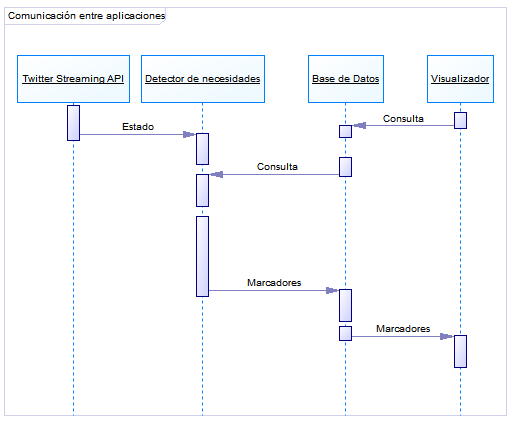
\includegraphics[scale=0.8]{images/ComunicacionFinal.png}
	\caption[Esquema que representa la comunicación entre aplicaciones del sistema detector de necesidades.]{Esquema que representa la comunicación entre aplicaciones del sistema detector de necesidades.\\Fuente: Elaboración Propia, (2016)}
	\label{fig:comunFinal}
\end{figure}

El módulo de detección comienza a recibir datos desde el \textit{stream} de \textit{Twitter} cuando el sistema es activado, luego el módulo de detección realiza consultas a la base de datos buscando si es que el usuario ha hecho ingreso de nuevos términos para filtrar la información entrante. Paralelamente, el módulo de visualización almacena los términos de búsqueda que hayan sido señalados por el usuario. Mientras tanto, el proceso de detección de necesidades continúa. Al concluir el proceso y obtener la respuesta, ésta es utilizada para generar nuevos marcadores, correspondientes a eventos donde se detectaron necesidades, los que pasan a ser almacenados en la base de datos. Periódicamente, el módulo de visualización realiza consultas a la base de datos, por medio de las cuales obtiene todos los nuevos marcadores generados desde la última consulta y los despliega en el mapa de la interfaz.

\subsection{Persistencia}
\label{sec:diseno:persistencia}

Anteriormente, se decidió la implementación de un sistema de persistencia en la aplicación para almacenar la información generada por esta, pero no se ha definido cuál ha de ser el sistema de gestión de base de datos que se ha de utilizar, es por ello que esta sección se presenta el cómo se tomó una decisión con respecto a este punto.

Debido a que se requiere mantener una ventana de datos históricos, se requiere un mecanismo de persistencia o base de datos. Además, los datos han de ser almacenados, al menos durante un tiempo, para que el sistema pueda realizar la generación de estadísiticas con respecto a ellos.

Se consideraron los principales sistemas de bases de datos utilizados y conocidos por el autor, dentro de los cuales se encontraban herramientas relacionales como MySQL, PostgreSQL, SQL Server y MongoDB para el caso de sistemas de gestión de base de datos (DBMS) no relacionales. Dadas las características y las condiciones con las cuales opera el sistema de detección, se requiere de un DBMS con baja latencia en operaciones lectura/escritura. La decisión se tomó en base a como se manejan los datos, pues no se apreció necesidad de implementar una modelo relacional, dado que lo que se requiere es velocidad y no mantener consistencia relacional entre los datos. De esta forma y teniendo en cuenta los resultados presentados en pruebas realizadas por \cite{MongoPerformance}, en las cuales mostró que el tiempo de respuesta (en operaciones de lectura) es significativamente menor en MongoDB que en dos de los DBMS más conocidos como MySQL y PostgreSQL se consideró utilizar este DBMS. Lo anterior, sumado al hecho de la capacidad de escalar de MongoDB reportada en fuentes oficiales o por diversos desarrolladores como \cite{MongoDBScalability} que han compartido sus experiencias en la \textit{Web}, llevaron a decidir que MongoDB debiese ser el sistema de gestión de base de datos que se usase en el sistema.

Para realizar la conexión de MongoDB y el \textit{framework} se utiliza una bibliotecas especialmente diseñada para aquello que corresponde a un ORM (Mapeo Objeto-Relacional), denominado \textit{Jongo}\footnote{http://jongo.org/}, para realizar la conversión de objeto Java a JSON y viceversa.

Habiendo resuelto lo anterior la siguiente problemática que se presenta radica en qué informacion almacenar. Según la definición de la historia de usuario HU-v04 en la que se señalan ``eventos pasados dentro de un intervalo de tiempo", se infiere que ha de guardarse tanto el contenido visible del dato, la clasificación que se le asignó y la fecha en que se identificó, para ello y dado que se seleccionó MongoDB, se especificó un esquema para los documentos de la colección donde sólo resta tener la información correspondiente a la ubicación, por lo que el esquema se definió como se presenta en la Figura \ref{fig:esquemaMarker1} correspondiente a la colección ``Markers".

\begin{figure}[H]
	\centering
	\captionsetup{justification=centering}
	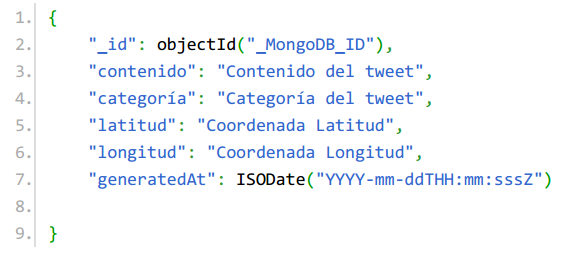
\includegraphics[scale=0.8]{images/Marker1.png}
	\caption[Ejemplo de documento en la colección Markers.]{Ejemplo de documento en la colección Markers.\\Fuente: Elaboración Propia, (2016)}
	\label{fig:esquemaMarker1}
\end{figure}

El primer campo corresponde al ID asignado por \textit{Mongo} para cumplir con la unicidad de los datos, el segundo campo corresponde al contenido textual del \textit{tweet} para ser mostrado junto con el marcador y que el usuario pueda ver desde dónde el sistema asignó aquel \textit{tweet} a una categoría en particular. El tercer campo corresponde al nombre de la etiqueta o categoría asignada al \textit{tweet}, esta asignación está dada por el resultado de la evaluación del clasificador. Los campos cuarto y quinto corresponden a la ubicación geográfica en la que se posiciona el marcador (latitud y longitud), y finalmente, el sexto campo corresponde al momento en que fue creado el marcador para ser utilizado en los diferentes criterios de visualización del sistema (relacionados a la HU-v08).

\subsection{Sistema de procesamiento}
\label{sec:diseno:sistDeProce}

Dado el contexto del funcionamiento del sistema, este ha de entregar respuestas rápidas ante una emergencia. Para ello, y como es descrito en la historia de usuario HU-c00, se requiere de un sistema capaz de procesar eventos en tiempo real que dada la masividad de datos con los que debe lidiar la aplicación, pueda escalar. El problema en este punto es el cómo construir un sistema capaz de identificar necesidades y que posea esta propiedad.

Se consideraron sistemas de procesamiento distribuido \textit{Apache S4}, \textit{Apache Storm} y \textit{Apache Spark}. Estos sistemas tienen la particularidad de poder trabajar con múltiples máquinas. 

Apache S4, pese a su simplicidad, no continuó con su desarrollo luego del año 2013 y nunca tuvo una versión estable ``1.0", razones por las cuales no se consideró como primera opción. Apache Spark, pese a contar con continuos \textit{releases}, una comunidad de desarrolladores no menor y permitir la elaboración de sistemas escalables no era lo que se buscaba en aquel momento como herramienta de desarrollo, pues está orientado al procesamiento por lotes y no en tiempo real. Al momento de consultar con los clientes, estos esperaban que el sistema, internamente, se comportara según el paradigma de procesamiento de \textit{streams}, por medio de operadores dispuestos en un grafo. Por ello finalmente se optó por \textit{Apache Storm}.

\textit{Storm} permite construir sistemas que cumplan con las características de un sistema distribuido, como lo son: escalabilidad (tanto horizontal como vertical) y tolerancia a fallos (como la capacidad de un sistema para realizar correctamente y en todo momento aquello para lo que fue diseñado). Estos sistemas están compuestos por dos tipos de elementos: \textit{Spout} y \textit{Bolt}, descritos en el Capítulo \ref{cap:MarcTeorico}. Al combinar esos elementos se da origen a un grafo dirigido, como el presentado en la Figura \ref{fig:stormBeLike} donde cada elemento de procesamiento (\textit{Bolt}), cumple con una determinada tarea recibiendo como entrada la salida del elemento de nivel anterior.

\subsection{Fuente de datos}
\label{sec:diseno:obtenerDatos}

La historia de usuario HU-c01 refleja desde dondé se han de obtener los datos, pero es necesario especificar aún más la forma en la que se obtienen. Como se señaló al momento de definir los alcances de este trabajo, sólo se utiliza \textit{Twitter} como fuente de información, así la unidad básica de información son los \textit{Tweet}.

Existen tres tipos de \textit{streaming endpoints} disponibles para obtener la información, cada uno para un caso de uso particular y son descritos en la Tabla \ref{tab:StreamingEndpoints}.

\begin{table}[H]
\centering
\caption[\textit{Streaming endpoints} de \textit{Twitter}.]{\textit{Streaming endpoints} de \textit{Twitter}.\\Fuente: Elaboración Propia, (2016)}
\label{tab:StreamingEndpoints}
\begin{tabular}{|l|l|}
\hline
Público & \begin{tabular}[c]{@{}l@{}}Stream del que fluye la información pública de Twitter.\\ Casos de uso: Seguimiento de usuarios o tópicos específicos o minería de datos.\end{tabular} \\ \hline
Usuario & Flujo que toda la información correspondiente a un usuario.                                                                                                                       \\ \hline
Sitio   & Versión multi-usuario de la anterior.                                                                                                                                             \\ \hline
\end{tabular}
\end{table}

Para esta aplicación corresponde hacer uso de la API pública. En ésta, a la vez, existen dos puntos de acceso, el acceso público y \textit{firehose}. El acceso público es gratuito y permite el acceso a un 1\% de la información que se genera en tiempo real y para acceder a el basta con crear una aplicación dentro de \textit{Twitter}. En cambio para acceder a \textit{firehose}, el cual permite acceso total a la información, debe comprarse el acceso. Dadas estas condiciones se seleccionó, previo acuerdo con los clientes, el uso de la API pública.

Para hacer uso de la API descrita con anterioridad es necesario obtener cuatro claves de acceso: \textit{Access Token}, \textit{Access Token Secret}, \textit{Consumer Key (API Key)} y \textit{Consumer Secret (API Secret)}. En el \ref{apendice:clavesApi} se incluye más información sobre cómo conseguir estas claves.

\subsection{Términos de búsqueda}
\label{sec:diseno:termBusqueda}

\textit{Twitter4J}\footnote{http://twitter4j.org/}, es una herramienta que permite obtener el flujo de información desde \textit{Twitter} e implementa una forma de filtrado mediante el uso de palabras clave. Sin embargo, la herramienta posee una limitante al momento de realizar modificaciones sobre este filtro, deben instanciarse nuevamente los objetos con los cuales se realiza la conexión a la API de \textit{Twitter}, es decir, volver a instanciar y conectar el \textit{Spout}, eso se traduce en tiempo de procesamiento perdido. Para solucionar este inconveniente se decidió implementar un operador, descrito en la sección \ref{subsec:detectorNecesidades}, el cual está encargado de realizar el filtrado de acuerdo a términos y llevar a cabo la operaciones descritas en la sección \ref{subsubsec:2op} referente a la expansión de la consulta. Sin embargo, un operador como este puede poseer réplicas que operan al mismo tiempo, con esto surge el problema de cómo comunicar y aplicar los nuevos términos de búsqueda y desechar los antiguos.

Para dar solución a esta problemática, se decidió recurrir a la base de datos, almacenar la consulta y asignar un estado para controlar el comportamiento del operador. Así, el esquema en la base de datos queda tal y como se presenta en la Figura \ref{fig:esquemaQuery}, documento de la colección ``Queries".

\begin{figure}[H]
	\centering
	\captionsetup{justification=centering}
	\includegraphics[scale=0.8]{images/Query.png}
	\caption[Ejemplo de documento en la colección queries.]{Ejemplo de documento en la colección queries.\\Fuente: Elaboración Propia, (2016)}
	\label{fig:esquemaQuery}
\end{figure}

La propiedad ``estado" del documento de la colección ``queries" puede tomar dos valores: ``actual" o ``antiguo", reflejando si una consulta se está llevando a cabo o no. Estos valores son asignados por la aplicación responsable de la interfaz, la encargada de recibir los términos de búsqueda por parte del usuario.

Para implementar este operador se desarrollaron dos clases llamadas \textit{CurrentQueryChecker} y \textit{QueryExpander}. La primera, para detectar cuándo y si es que ha cambiado una consulta en la base de datos y la segunda para desarrollar la labor descrita por el algoritmo de expansión presentado en la sección \ref{subsubsec:2op}.

\subsection{Categorización de necesidades}
\label{sec:diseno:categorias}

La definición de las categorías es un punto importante dentro de la construcción de la aplicación. Teóricamente, el tamaño del conjunto de entrenamiento ha de ser mayor o menor dependiendo de la cantidad de clases (categorías). 

Inicialmente, se consideró la taxonomía definida por \cite{TaxonomiaChato}, pero el equipo del proyecto FONDEF estableció que no era conveniente utilizarla, pues presentaba gran cantidad de categorías y era demasiado específica. Como alternativa se sugirió utilizar la clasificación realizada por \cite{PMIProfes}, en la que se presenta una categorización de cinco categorías. Esta categorización se realizó por parte de un equipo de psicólogos expertos en el contexto del proyecto PMI-USA 1204, basándose en la información obtenida del terremoto de febrero de 2010 y los \textit{tweets} recolectados en dicho evento. Esta categorización está compuesta de las siguientes categorías:

\begin{enumerate}
\item Necesidades básicas: \textit{tweet} que entrege o solicite información sobre serviciós básicos: Agua potable, electricidad y abastecimiento de alimentos.
\item Comunicación: \textit{tweet} que entregue o solicite información sobre alguna localidad.
\item Seguridad: \textit{tweet} que señale un riesgo para la población.
\item Personas: \textit{tweet} que haga referencia al hallazgo o búsqueda de una persona desaparecida.
\item Irrelevante: cualquier otro \textit{tweet}.
\end{enumerate}

Acordando con el equipo, se decidió separar el primer ítem en los tres elementos que lo componen: Agua, alimentos y electricidad. Así, finalmente, se obtienen las siete categorías que se utilizan en el sistema.\\

Los elementos clasificados como ``Irrelevantes" no se muestran en el mapa de eventos, pues hacen referencia a eventos que, pese a haber pasado por todos los operadores anteriormente descritos, no guardan relación con el evento o sus consecuencias. Estos pueden ser \textit{tweets} a etiquetar por expertos \textit{a posteriori} con el objetivo de enriquecer la información del clasificador. Sin embargo, esta tarea está fuera del alcance de este proyecto.

\subsection{Clasificador}
\label{sec:diseno:clasificador}

Se busca generar un clasificador automático capaz de detectar necesidades y lidiar con la jerga nacional. Para ello, según lo descrito por \cite{IRQE} en su libro \textit{Introduction to Information Retrival}, se entrenó un clasificador basado en \textit{Naïve Bayes}, haciendo uso de Mallet, pues presenta mejores resultados en la predicción que RapidMiner y Weka.

La sección \ref{sec:caracteristicasSistema} ya hace referencia a la inconveniencia de utilizar un clasificador estático para el etiquetado de nuevos eventos, al tratarse de un aprendizaje supervisado, donde se requiere de una persona entregue la respuesta esperada para realizar el entrenamiento, no es posible realizar este proceso de manera automática.

Al no poder automatizar el proceso antes señalado se consultó con el equipo del proyecto FONDEF IDeA si es que era factible la implementación de un actualizador manual del clasificador, lo cual fue aceptado.

Segun la metodologia KDD, los pasos que se siguen para construir un nuevo clasificador son los siguientes:

Los datos son seleccionados por el usuario, estos datos se agruparan en un archivo de texto, un archivo CSV en el cual los elementos se separaran utilizando el caracter punto y coma (;). El formato que se utiliza para el archivo de entrada se muetra en la Figura \ref{fig:formatoFig} , así cualquier archivo que cumpla con el formato permite la creación de un nuevo modelo clasificador.

\begin{figure}[H]
	\centering
	\captionsetup{justification=centering}
	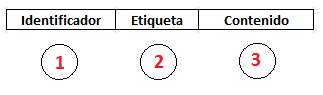
\includegraphics[scale=0.8]{images/FormatoArchivoEntrada.png}
	\caption[Formato archivo de entrada.]{Formato archivo de entrada.\\Fuente: Elaboración Propia, (2016)}
	\label{fig:formatoFig}
\end{figure}

\begin{enumerate}
\item Corresponde a un identificador arbitrario, pero necesario para la herramienta de clasificación Mallet.
\item Corresponde a la etiqueta que categoriza al contenido.
\item Contenido del \textit{tweet} propiamente tal.
\end{enumerate}

El preprocesamiento y transformación de los datos se realiza utilizando los operadores de transformación (normalizador de texto, eliminación de \textit{stopwords} y proceso de \textit{stemming}), presentados en la sección \ref{subsec:detectorNecesidades}.

Teniendo en consideración que se utilizan dos módulos distintos, donde en uno se construye el clasificador y es utilizado en el otro módulo, surge el problema de cómo realizar la comunicación entre ellos. Para solucionar este inconveniente se utiliza una carpeta compartida por ambas aplicaciones. En el caso de sistemas Unix se utiliza el directorio $/opt/DeNe$, mientras que para Windows se utiliza $C:/DeNe/$. En estos directorios se almacena un fichero con el clasificador serializado.

\begin{figure}[H]
	\centering
	\captionsetup{justification=centering}
	
\includegraphics[scale=0.8]{images/ClasifierDene.png}
	\caption[Fichero clasificador en $c:/DeNe/$.]{Fichero clasificador en $C:/DeNe/$.\\Fuente: Elaboración Propia, (2016)}
	\label{fig:TopologiaGeneral}
\end{figure}

Cada vez que se actualice el clasificador se contrasta el nuevo con el ya existente. En el caso de encontrar mayor precisión en el primero, se reemplaza en las carpetas antes mencionadas, según el sistema operativo de la máquina que se esté utilizando. En caso contrario, se mantiene el anterior. En ambos escenarios se le da a conocer al usuario la precisión de ambos.

\subsection{Interfaz web}
\label{sec:diseno:interfaz}

Teniendo en consideración la característica del desarrollo de esta aplicación como un proyecto ágil con un mínimo de personal de desarrollo se requería de un \textit{framework} que contribuyera a acelerar la construcción de la aplicación. Tras considerar las alternativas más conocidas como \textit{Spring}, \textit{Hibernate} o \textit{JSF} que tienen una curva de aprendizaje elevada, se optó por utilizar un cuarto \textit{framework} que aunque desconocido, promete una simplicidad en su uso. \textit{Play Framework}\footnote{https://www.playframework.com/}, construido haciendo uso de Scala y Java permite construir aplicaciones ligeras (tamaño en disco), sin estado (no guarda configuraciones de una sesión para ser utilizadas luego) y por defecto RESTful, ideal para la comunicación entre aplicaciones. Este \textit{framework} sigue el patrón de arquitectura Modelo-Vista-Controlador (MVC) y Cuenta con un compilador en tiempo real (compila y realiza el despliegue de la aplicación cuando detecta un cambio en el código), lo que agiliza en gran medida el desarrollo, pues al automatizar este proceso mantiene la atención en lo que se está desarrollando.

Para visualizar los puntos encontrados por el detector de necesidades se decidió utilizar la API de \textit{Google Maps} la que permite la colocación de los denominados ``marcadores" en un punto específico del mapa y asociar a ellos algún tipo de información. Así, aunque el funcionamiento interno esté dirigido por \textit{Play}, la principal funcionalidad del sistema, mostrar el mapa con sus marcadores, es implementada por medio de Javascript haciendo uso de esta API.

Los marcadores, ya ubicados en el mapa, tienen asociado un cuadro de texto dentro del cual refleja el la categoría a la que pertenece y el \textit{tweet} original que lo generó. La Figura \ref{fig:EjemploMarker} presenta un ejemplo de este funcionamiento en la interfaz \textit{Web}. La visualización del contenido del \textit{tweet} tiene como objetivo permitir decidir, en última instancia, al usuario si ha sido correctamente clasificado.

\begin{figure}[H]
	\centering
	\captionsetup{justification=centering}
	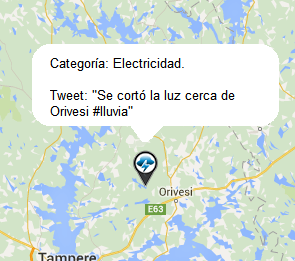
\includegraphics[scale=0.8]{images/EjemploMarker.png}
	\caption[Ejemplo de marcador en el mapa con su categorización y \textit{tweet} que lo generó.]{Ejemplo de marcador en el mapa con su categorización y \textit{tweet} que lo generó.\\Fuente: Elaboración Propia, (2016)}
	\label{fig:EjemploMarker}
\end{figure}

Según lo solicitado en la historia de usuario HU-v02 se prepararon dos tipos de filtros a la interfaz para la visualización de eventos en el mapa: El primero considera el agrupamiento o \textit{clustering} de marcadores, mientras que el segundo considera el tipo de marcador o marcadores que se desean visualizar.

Para el caso del agrupamiento se definieron tres modos de funcionamiento los cuales se describen a continuación:

\begin{enumerate}
\item No agrupar: Mostrar todos los marcadores que correspondan en el mapa de acuerdo al punto geográfico que corresponda en su definición.
\item Agrupar por distancia: Define una grilla invisible en el mapa donde los elementos que calcen en una cudrícula son agregados a un \textit{cluster} y visualizados como tal.
\item Agrupar por categoría: De igual forma que el agrupamiento por distancia, pero sólo agrega elementos que comparan categoría.
\end{enumerate}

La Figura \ref{fig:EjemploAmbosClusters} presentan un ejemplo de ambos tipos de agrupamiento especial, respectivamente por distancia y categoría.

\begin{figure}[H]
\centering
\captionsetup{justification=centering}
\subfloat[Cluster distancias.]{\centering\label{fig:mdleft}{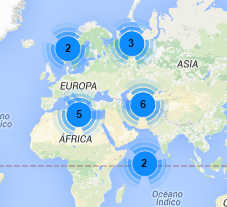
\includegraphics[width=0.45\textwidth]{images/EjemploCluster.png}}}\hfill
\subfloat[Cluster categoría.]{\centering\label{fig:mdleft}{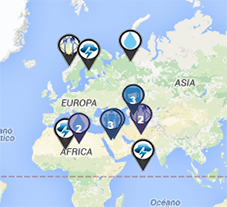
\includegraphics[width=0.45\textwidth]{images/ClusterCategoria.png}}}
\caption[Ejemplos de agrupamiento basados en distancia y categorías.]{Ejemplos de agrupamiento basados en distancia y categorías.\\Fuente: Elaboración Propia, (2016)}
\label{fig:EjemploAmbosClusters}
\end{figure}

Para el segundo caso sólo se definieron dos reglas de funcionamiento las cuales se describen a continuación:

\begin{enumerate}
\item Mostrar todos: Muestra elementos de todas las categorias existentes.
\item Mostrar categoría: Para cada categoría mostrar sólo los elementos de aquella categoría. 
\end{enumerate}

Al combinar ambos tipos de filtros se tienen potencialmente seis modos de funcionamiento, pero considerando las categorías descritas en al sección \ref{sec:diseno:categorias} ese número se expande a veintidós modos de funcionamiento del visualizador.

\section{Implementación del sistema}
\label{sec:implementacion}

En la presente sección se detalla el proceso de implementación de la solución diseñada. Para ello se trabaja en paralelo en el desarrollo de ambos modulos: \textit{front-end} y \textit{back-end} bajo la metodologia XP, donde se generan versiones sucesivas de la solución, las cuales evolucionan de acuerdo a los requermientos del cliente.

\subsection{\textit{Front-end}}
\label{subsec:imp:visualizador}

La implementación del visualizador de eventos se realizó haciendo uso del \textit{framework} de Java \textit{Play}, el cual por defecto crea aplicaciones que siguen el patrón de diseño MVC, por lo tanto se tienen tres niveles dentro de la aplicación:

\begin{itemize}
\item Modelo: donde están los elementos que permiten interactuar con la base de datos. 
\item Controlador: presentando los métodos de reacción ante los eventos detonados en el nivel de presentación.
\item Vista o presentación: muestra las interfaces \textit{Web} diseñadas para que el usuario interactúe con el sistema.
\end{itemize}

\subsubsection*{Filtrado de marcadores}
\label{subsubsec:filtradoMarcadores}

Dentro del nivel de presentación se encuentra el mapa proporcionado por la API de Google Maps como se mencionó en la sección \ref{sec:diseno:interfaz}. Allí se señaló que existen filtros para la visualización de eventos de manera que se la presentación de estos se apegue a las necesidades del usuario. Para implementar estos filtros, internamente la aplicación hace uso de $n + 1$ \textit{clusters}, donde $n$ corresponde al número de categorías y el cluster extra es para agruparlos a todos. Así, en el caso de querer ver los eventos agrupados, y dependiendo si se quiere o no agruparlos discriminando su categoría, se llenan los \textit{clusters} pertenecientes a la visualización general o a la visualización por categoría. Para el caso de querer mostrar sólo una categoría en particular, sólo se permite que los \textit{cluster} se llenen con los elementos de la categoría seleccionada. El Algoritmo \ref{alg:filtroMarcadores} presenta lo anteriormente descrito para facilitar la comprensión de la lógica interna de los filtros presentados.\\

\begin{algorithm}[H]\setstretch{1.5}
	\begin{algorithmic}[numeracion_lineas]
		\REQUIRE Tipo de agrupamiento $A$.
		\REQUIRE Discriminador de categoría $K$.
		\REQUIRE Marcadores $M$.
		\STATE Lista de marcadores $L$.
		\STATE \textit{Clusters} de marcadores $C = \{c_{0}, \dots, c_{n+1} \}$.
		\FOR{cada $m_{i}$ perteneciente a $M$}
			\IF{la categoría de $m_{i}$ no es ``irrelevante" y la categoría de $m_{i}$ es igual a $K$}
				\STATE añadir el marcador a $L$.
			\ELSIF{$K$ es ``todas las categorías"}
				\STATE añadir el marcador a $L$.
			\ENDIF
		\ENDFOR
		\IF{$A$ es ``no agrupar"}
			\FOR{cada $l_{i}$ perteneciente a $L$}
				\STATE posicionar $l_{i}$ en el mapa.
			\ENDFOR
		\ELSIF{$A$ es ``agrupar todos"}
			\FOR{cada $l_{i}$ perteneciente a $L$}
				\STATE añadir $l_{i}$ al clister $c_{0}$.
			\ENDFOR
			\STATE posicionar $c_{0}$ en el mapa.
		\ELSE
			\FOR{cada $l_{i}$ perteneciente a $L$}
				\STATE añadir $l_{i}$ al cluster $c_{i+1}$
			\ENDFOR
			\FOR{cada $c_{i}$ perteneciente a $C - \{c_{0}\}$}
				\STATE añadir $l_{i}$ al cluster $c_{i}$
			\ENDFOR
		\ENDIF
	\end{algorithmic}
	\caption{Algoritmos de utilización de filtros}
	\label{alg:filtroMarcadores}
\end{algorithm}\vphantom\\

Para realizar la selección del intervalo mencionado en la HU-v04 se solicitó, por parte del equipo FONDEF IDeA, el uso de una línea de tiempo con intervalo deslizante que, además, mostrase la cantidad de eventos detectados por fecha por medio de un histograma. Para ello se utilizó inicialmente \textit{JDateRangeSlider}, de la biblioteca Javascript \textit{JQRangeSlider}\footnote{http://ghusse.github.io/jQRangeSlider/}, \cite{JQRangeSlider}. Esta biblioteca era suficiente para seleccionar el intervalo de fechas y detectar cambios producidos en la línea de tiempo para actualizar los valores, mas no permite la implementación de un histograma externo.

\begin{figure}[H]
	\centering
	\captionsetup{justification=centering}
	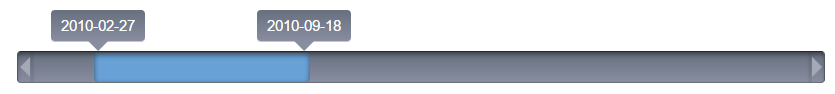
\includegraphics[scale=0.6]{images/JDateRangeSlider.png}
	\caption[Selectorde fechas JDateRangeSlider.]{Selectorde fechas JDateRangeSlider.\\Fuente: \cite{JQRangeSlider}}
	\label{fig:JQRangeSlider}
\end{figure}

Para lograr implementar ambas funcionalidades, línea de tiempo e histograma, se utilizó una biblioteca Javascript distinta. La Figura \ref{fig:HistogramaFinal} presenta la implementación utilizando \textit{HighCharts}, \cite{Highcharts}. Esta biblioteca, al contrario de \textit{JQRangeSlider}, no permitía capturar los cambios en el histograma para reaccionar cuando se produjese un cambio en él. Para solucionar este inconveniente se implementó una función Javascript que recogiese los valores actuales del intervalo y arrojase un evento cuando se produjece un cambio. Este evento se asoció al eje x de la línea temporal. De esta manera, cada vez que se modifiquen los valores del eje se dispare un nuevo evento, el que pasa a ser capturado y produce la actualización de los marcadores del mapa. La implementación del disparador de este evento es descrito en la Figura \ref{fig:implementacionCambiosEnEje}.

\begin{figure}[H]
	\centering
	\captionsetup{justification=centering}
	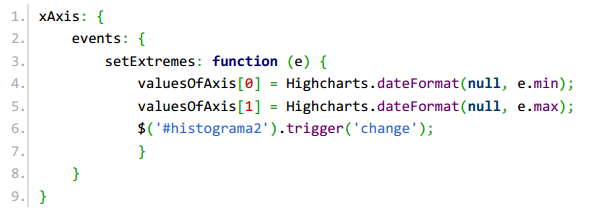
\includegraphics[scale=0.8]{images/onChangeEventTimeline.png}
	\caption[Implementación de evento de detección de cambios en la línea temporal.]{Implementación de evento de detección de cambios en la línea temporal.\\Fuente: Elaboración Propia, (2016)}
	\label{fig:implementacionCambiosEnEje}
\end{figure}

Inicialmente este histograma sólo está disponible en inglés, pero permite cambiar todas sus etiquetas manualmente. Así, para mejorar la usabilidad de la aplicación se modificaron todos los textos para estuviesen en español. El resultado de esta modificación es presentado en la Figura \ref{fig:HistogramaFinal}.

\begin{figure}[H]
	\centering
	\captionsetup{justification=centering}
	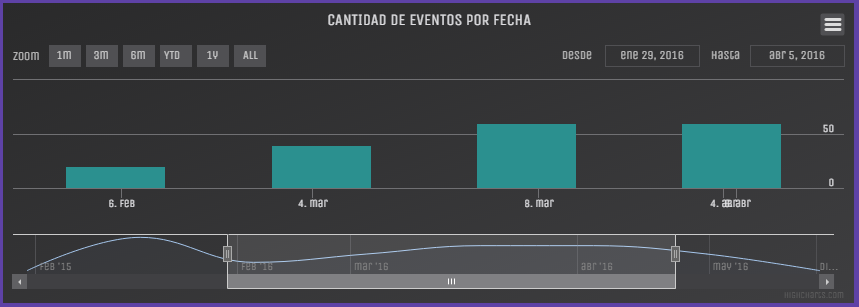
\includegraphics[scale=0.6]{images/Histograma.png}
	\caption[Selector de fechas presente en la aplicación.]{Selector de fechas presente en la aplicación.\\Fuente: Elaboración Propia, (2016)}
	\label{fig:HistogramaFinal}
\end{figure}

Tras la selección de intervalo dentro del cual se desea que el sistema muestre los estados recibidos, se realiza una consulta del tipo POST con parámetros fecha inicial y final, para obtener una lista con todos los marcadores encontrados en ese rango.

Los iconos correspondientes a las categorías que soporta el sistema se definieron mediante la combinación de dos imágenes para cada categoría: un marcador de mapa, similar a los definidos en la API de Google Maps y una que sugiriera al usuario la categoría a la que hace referenciar. Los diseños finales son presentados en la Figura \ref{fig:categoriasFig}

\begin{figure}[H]
\centering
\subfloat[Categoría agua.]{
	\makebox[4cm][c]{
		\label{fig:mdleft}{
			
\includegraphics[width=1.5cm]{images/categorias/agua.png}
		}
	}
}\hfill
\subfloat[Categoría alimento.]{
	\makebox[4cm][c]{
		\label{fig:mdleft}{
			
\includegraphics[width=1.5cm]{images/categorias/alimento.png}
		}
	}
}\hfill
\subfloat[Categoría electricidad.]{
	\makebox[4cm][c]{
		\label{fig:mdright}{
			
\includegraphics[width=1.5cm]{images/categorias/electricidad.png}
		}
	}
}\hfill
\vfill
\subfloat[Categoría comunicación]{
	\makebox[4cm][c]{
		\label{fig:mdleft}{
			
\includegraphics[width=1.5cm]{images/categorias/comunicacion.png}
		}
	}
}\hfill
\subfloat[Categoría personas.]{
	\makebox[4cm][c]{
		\label{fig:mdleft}{
			
\includegraphics[width=1.5cm]{images/categorias/personas.png}
		}
	}
}\hfill
\subfloat[Categoría seguridad.]{
	\makebox[4cm][c]{
		\label{fig:mdright}{
			
\includegraphics[width=1.5cm]{images/categorias/seguridad.png}
		}
	}
}\hfill
\caption[Categorías para marcadores.]{Iconos de categorías para marcadores.\\Fuente: Elaboración Propia, (2016)}
\label{fig:categoriasFig}
\end{figure}

Además, se consideró apropiado diseñar un icono que representara la densidad de marcadores al momento de realizar el agrupamiento por categorías descrito en esta sección, para ello y siguiendo la combinación de colores utilizada por la biblioteca \textit{MarkerClusterer} donde se muestra un cluster azul cuando es un cluster pequeño; amarillo para uno medio y rojo para uno grande, \cite{MarkerClusterer}. La definición de estos colores es descrita a continuación:

\begin{itemize}
\item Azul: De dos a diez elementos.
\item Amarillo: De once a cien elementos amarillo.
\item Rojo: Desde cien elementos.
\end{itemize}

Se prepararon tres iconos adicionales a cada categoría para reemplazar los íconos por defecto de la biblioteca, las que pueden verse en las Figuras \ref{fig:clusterAgua}. a la \ref{fig:clusterseguridad}.

\begin{figure}[H]
\centering
\subfloat[Cluster pequeño.]{
	\makebox[4cm][c]{
		\label{fig:mdleft}{
			
\includegraphics[width=1.5cm]{images/categorias/aguaS.png}
		}
	}
}\hfill
\subfloat[Cluster medio.]{
	\makebox[4cm][c]{
		\label{fig:mdleft}{
			
\includegraphics[width=1.5cm]{images/categorias/aguaM.png}
		}
	}
}\hfill
\subfloat[Cluster grande.]{
	\makebox[4cm][c]{
		\label{fig:mdright}{
			
\includegraphics[width=1.5cm]{images/categorias/aguaL.png}
		}
	}
}
\caption[Iconos de cluster para categoría agua.]{Iconos de cluster para categoría agua.\\Fuente: Elaboración Propia, (2016)}
\label{fig:clusterAgua}
\end{figure}

\begin{figure}[H]
\centering
\subfloat[Cluster pequeño.]{
	\makebox[4cm][c]{
		\label{fig:mdleft}{
			
\includegraphics[width=1.5cm]{images/categorias/alimentoS.png}
		}
	}
}\hfill
\subfloat[Cluster medio.]{
	\makebox[4cm][c]{
		\label{fig:mdleft}{
			
\includegraphics[width=1.5cm]{images/categorias/alimentoM.png}
		}
	}
}\hfill
\subfloat[Cluster grande.]{
	\makebox[4cm][c]{
		\label{fig:mdright}{
			
\includegraphics[width=1.5cm]{images/categorias/alimentoL.png}
		}
	}
}
\caption[Iconos de cluster para categoría alimento.]{Iconos de cluster para categoría alimento.\\Fuente: Elaboración Propia, (2016)}
\label{fig:clusteralimento}
\end{figure}

\begin{figure}[H]
\centering
\subfloat[Cluster pequeño.]{
	\makebox[4cm][c]{
		\label{fig:mdleft}{
			
\includegraphics[width=1.5cm]{images/categorias/electricidadS.png}
		}
	}
}\hfill
\subfloat[Cluster medio.]{
	\makebox[4cm][c]{
		\label{fig:mdleft}{
			
\includegraphics[width=1.5cm]{images/categorias/electricidadM.png}
		}
	}
}\hfill
\subfloat[Cluster grande.]{
	\makebox[4cm][c]{
		\label{fig:mdright}{
			
\includegraphics[width=1.5cm]{images/categorias/electricidadL.png}
		}
	}
}
\caption[Iconos de cluster para categoría electricidad.]{Iconos de cluster para categoría electricidad.\\Fuente: Elaboración Propia, (2016)}
\label{fig:clusterelectricidad}
\end{figure}

\begin{figure}[H]
\centering
\subfloat[Cluster pequeño.]{
	\makebox[4cm][c]{
		\label{fig:mdleft}{
			
\includegraphics[width=1.5cm]{images/categorias/comunicacionS.png}
		}
	}
}\hfill
\subfloat[Cluster medio.]{
	\makebox[4cm][c]{
		\label{fig:mdleft}{
			
\includegraphics[width=1.5cm]{images/categorias/comunicacionL.png}
		}
	}
}\hfill
\subfloat[Cluster grande.]{
	\makebox[4cm][c]{
		\label{fig:mdright}{
			
\includegraphics[width=1.5cm]{images/categorias/comunicacionL.png}
		}
	}
}
\caption[Iconos de cluster para categoría comunicación.]{Iconos de cluster para categoría comunicación.\\Fuente: Elaboración Propia, (2016)}
\label{fig:clustercomunicacion}
\end{figure}

\begin{figure}[H]
\centering
\subfloat[Cluster pequeño.]{
	\makebox[4cm][c]{
		\label{fig:cluster}{
			
\includegraphics[width=1.5cm]{images/categorias/personasS.png}
		}
	}
}\hfill
\subfloat[Cluster medio.]{
	\makebox[4cm][c]{
		\label{fig:mdleft}{
			
\includegraphics[width=1.5cm]{images/categorias/personasM.png}
		}
	}
}\hfill
\subfloat[Cluster grande.]{
	\makebox[4cm][c]{
		\label{fig:mdright}{
			
\includegraphics[width=1.5cm]{images/categorias/personasL.png}
		}
	}
}
\caption[Iconos de cluster para categoría personas.]{Iconos de cluster para categoría personas.\\Fuente: Elaboración Propia, (2016)}
\label{fig:clusterpersonas}
\end{figure}

\begin{figure}[H]
\centering
\subfloat[Cluster pequeño.]{
	\makebox[4cm][c]{
		\label{fig:mdleft}{
			
\includegraphics[width=1.5cm]{images/categorias/seguridadS.png}
		}
	}
}\hfill
\subfloat[Cluster medio.]{
	\makebox[4cm][c]{
		\label{fig:mdleft}{
			
\includegraphics[width=1.5cm]{images/categorias/seguridadM.png}
		}
	}
}\hfill
\subfloat[Cluster grande.]{
	\makebox[4cm][c]{
		\label{fig:mdright}{
			
\includegraphics[width=1.5cm]{images/categorias/seguridadL.png}
		}
	}
}
\caption[Iconos de cluster para categoría seguridad.]{Iconos de cluster para categoría seguridad.\\Fuente: Elaboración Propia, (2016)}
\label{fig:clusterseguridad}
\end{figure}

Dado que se solicitó que la interfaz no se recargue cada vez que se produzca un cambio dado por un nuevo evento detectado o la modificación en el intervalo de visualización, se utilizaron las tecnologías Javascript y AJAX para capturar los cambios en la línea temporal al momento de su ocurrencia, descrita en esta sección. Cada vez que se detecte un cambio, se elimina todo marcador del mapa y se reubican en el todos los que cumplan con los parámetros de búsqueda sin necesidad de refrescar la página completa.

\subsubsection*{Estadísticas de procesamiento}
\label{subsubsec:estadisticasdeproc}

Específicamente se solicitaron tres tipos de estadísticas que han de ser mostradas por consulta, estas se definen a continuación:

\begin{enumerate}
\item Cantidad de eventos detectados, es decir, \textit{tweets} que fueron clasificados.
\item Cantidad de usuarios distintos identificados en aquellos eventos.
\item Cantidad total de \textit{tweets} que han pasado por el sistema desde el inicio de la consulta actual.
\end{enumerate}

Para cumplir lo solicitado se necesitaba añadir elementos no considerados en la base de datos; hace falta conocer al usuario y contar los \textit{tweets} ingresados desde \textit{Twitter4J}.

Para completar esta historia se realizaron modificaciones al esquema previamente definido en la sección \ref{sec:diseno:persistencia}, este de por sí era suficiente para cumplir con la estadística número uno, pero incapaz de realizar las otras dos. Para la segunda estadística se consideró que bastaba con guardar al usuario junto con la colección de marcadores. De acuerdo a \cite{TwitterAgreement} en su sección F. \textit{Be a Good Partner to Twitter}, se insta a los desarrolladores que almacenen contenido \textit{offline} de \textit{Twitter}, a almacenar sólo el ID del usuario o del \textit{tweet}, por ello y siguiendo estos lineamientos se agrega el campo ``userID" al esquema marcadores, pasando a quedar como se aprecia en la Figura \ref{fig:esquemaMarker2}.

\begin{figure}[H]
	\centering
	\captionsetup{justification=centering}
	\includegraphics[scale=0.8]{images/Marker2.png}
	\caption[Ejemplo de documento en la colección Markers.]{Ejemplo de documento en la colección Markers.\\Fuente: Elaboración Propia, (2016)}
	\label{fig:esquemaMarker2}
\end{figure}

Para la tercera estadística la colección de marcadores no sería útil, pues no refleja la cantidad de tweets procesados, para ello es necesario implementar una tercera colección de documentos en la base de datos y almacenarlos antes de la aplicación de cualquier tipo de filtro. Esta colección tiene el esquema presente en la Figura \ref{fig:esquemaTweet}.

\begin{figure}[H]
	\centering
	\captionsetup{justification=centering}
	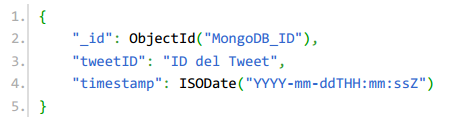
\includegraphics[scale=0.8]{images/status.png}
	\caption[Ejemplo de documento en la colección Status.]{Ejemplo de documento en la colección Status.\\Fuente: Elaboración Propia, (2016)}
	\label{fig:esquemaTweet}
\end{figure}

Al almacenar sólo el identificador del \textit{tweet} no viola las políticas de uso descritas de \textit{Twitter}, sólo es necesario la fecha para la estadística realizar la estadística. En general la obtención de estas estadísticas se realiza utilizando el Algoritmo \ref{alg:estadisticas}.\\

\begin{algorithm}[H]\setstretch{1.5}
	\begin{algorithmic}[numeracion_lineas]
		\REQUIRE Colección $c$ 
		\REQUIRE Fecha de la consulta actual $f$ 
		\ENSURE Contador de eventos $counter$  
		\STATE $counter = 0$
		\FOR{Documento $d_{i}$ en la colección $c$}
			\IF{ fecha de $d_{i}$ es posterior a $f$}
				\STATE $counter = counter + 1$
			\ENDIF	
		\ENDFOR
		\RETURN $counter$
	\end{algorithmic}
	\caption{Algoritmos de generación de primera y tercera estadística.}
	\label{alg:estadisticas}
\end{algorithm}\vphantom\\

Este algoritmo, como se mencionó, es de uso general y permite cumplir tanto la primera como la tercera estadística, para el caso de la segunda se requiere una modificación, pues se solicitó conocer los usuarios diferentes, el Algoritmo \ref{alg:estadisticas2} presenta el algoritmo modificado para la segunda estadística.\\

\begin{algorithm}[H]\setstretch{1.5}
	\begin{algorithmic}[numeracion_lineas]
		\REQUIRE Colección $c$ 
		\REQUIRE Fecha de la consulta actual $f$ 
		\ENSURE Lista de usuarios vacía $list$  
		\FOR{Documento $d_{i}$ en la colección $c$}
			\IF{ fecha de $d_{i}$ es posterior a $f$}
				\IF{ID del usuario de $d_{i}$ no está en $list$ o $list$ es vacía}
					\STATE Añadir $d_{i}$ a $list$
				\ENDIF
			\ENDIF	
		\ENDFOR
		\RETURN Cantidad de elementos en $list$
	\end{algorithmic}
	\caption{Algoritmos de generación de segunda estadísticas.}
	\label{alg:estadisticas2}
\end{algorithm}\vphantom\\

Para mostrar las estadísticas es necesario comunicar los datos al \textit{front-end} de la aplicación, para lo cual se utiliza el mismo principio utilizado para la actualización de los marcadores, en donde cada cierto tiempo se consulta a la base de datos por nuevos marcadores. Para el caso de las estadísticas se implementó un servicio de consulta del tipo GET para obtener, mediante AJAX, el valor del resultado de la implementación de los algoritmos expuestos anteriormente.

\subsubsection*{Configuración}
\label{subsubsec:config}

La necesidad de un segmento de configuración nace producto de la HU-v01. El visualizador de eventos tiene dos maneras de comportarse:

\begin{itemize}
\item Modo tiempo real: Cuando el sistema esté en funcionamiento y cada cierto tiempo, $t_{1}$, se actualizan los marcadores de los nuevos eventos y estos se muestran durante un tiempo, $t_{2}$.
\item Modo línea de tiempo: Funcionamiento basado en lo descrito en HU-v04.
\end{itemize}

Los tiempos $t_{1}$ y $t_{2}$ inicialmente fueron decididos de manera arbitraria, pero al mostrar su funcionamiento se sugirió que estos parámetros pudiesen ser definidos por el usuario. Por ello, se implementó una sección de configuración dentro de la aplicación de visualización para permitir la definición de estos valores. La importancia de la definición de estos valores viene dada por las necesidades del usuario, pero traen consecuencias al sistema.

Para el caso del tiempo $t_{1}$, un menor $t_{1}$ implica que se realizan más consultas al sistemas, pese a esto, es adecuado un valor pequeño cuando se encuentre en operación y el sistema de detección esté generando contenido constantemente. Para la operación en periodos normales, es decir, cuando no esté ocurriendo un evento del tipo desastre, la generación de eventos será nula o muy baja, en esas ocaciones es recomentable un $t_{1}$ elevado.

Para el caso del tiempo $t_{2}$, este está dado por el tiempo que el usuario estime que un evento se encuentra vigente. El valor de t2 no afecta de gran manera al sistema, pues sólo tiene fines visuales, descartando eventos que no cumplan con la ventana de tiempo $Tiempo actual - tiempo de creación \geq t_{2}$, a mayor $t_{2}$, mayor es la ventana de tiempo en la que un evento se considera vigente.

\subsection{Back-end}
\label{subsec:detectorNecesidades}

El detector de necesidades se implementa utilizando un motor de procesamiento de \textit{stream}, en este caso \textit{Storm}. La implementación de \textit{Storm} requiere de la definición de una topología de grafo compuesta por operadores que realizan tareas y comparten eventos. Para implementar el detector se requirió de la construcción de operadores especializados capaces de realizar alguna de las tareas necesarias para detectar las necesidades expresadas en el texto. A continuación se presenta la construcción de estos operadores.

\subsubsection*{Operador fuente de datos}
\label{subsubseC:EntradaDeDatos}

Este operador es el encargado de conectarse a la fuente de datos, en este caso la API de \textit{Twitter}, y comunicar los eventos resto del sistema de procesamiento de \textit{stream}. En el caso particular de \textit{Storm}, este operador corresponde a un \textit{Spout}.

Conociendo desde donde se obtiene la información y teniendo acceso a ella resta conocer cómo realizar la conexión. Para ello se decidió utilizar \textit{Twitter4J}, una biblioteca no oficial de Java para las API de \textit{Twitter}. Para su funcionamiento sólo requiere del uso de Java en su versión 5 o superior.

La implementación de lo anteriormente descrito se realiza utilizando una instancia del objeto \textit{TwitterStream}, el cual captura el flujo público de \textit{Twitter}, almacenando cada \textit{tweet} recibido en una cola. Con esto en mente se construyó el primer operador del sistema correspondiente al \textit{Spout} que surte de datos al sistema.

\begin{figure}[H]
	\centering
	\captionsetup{justification=centering}
	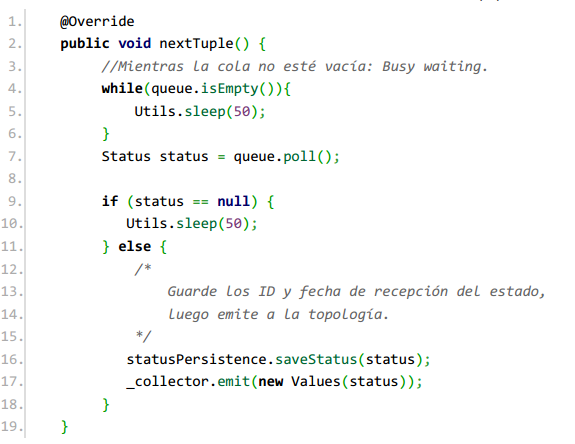
\includegraphics[scale=0.8]{images/TwitterSpout.png}
	\caption[Implementación del \textit{Spout} del sistema.]{Implementación del \textit{Spout} del sistema.\\Fuente: Elaboración Propia, (2016)}
	\label{fig:TwitterSpout}
\end{figure}

Considerando lo recién expuesto la Figura \ref{fig:TwitterSpout} muestra cómo los estados son emitidos por el \textit{spout} al sistema basándose en la cola (\textit{queue}) para manejar lo que llega desde el \textit{stream}. Al ser llamado por parte de \textit{Storm}, el método \textit{nextTuple} espera a que la cola de eventos no esté vacía y cuando esto se cumple toma un \textit{tweet} (\textit{status}) y lo emite al sistema, no sin antes almacenar su ``tweetID" con fines estadísticos.

\subsubsection*{Operador idioma}
\label{subsubsec:1op}

El presente trabajo se enfoca en la detección de necesidades en español. De acuerdo a \cite{TwitterActiveUsers}, existen actualmente 310 millones de usuarios activos en \textit{Twitter} (a enero del 2016), de los cuales 65 millones pertenecen a los Estados Unidos, cuyo idioma oficial es el inglés, según \cite{TwitterStats1}. Se estima que este año, en latinoamérica, Brasil, cuyo idioma oficial es el portugués, alcance los 15 millones de usuarios según \cite{TwitterStats2}, sin considerar paises árabes o asiáticos podemos deducir que al menos un 30\% de los usuarios activos de \textit{Twitter} hablan idiomas distintos al español. Dado que el sistema está pensado para operar dentro de Chile donde el idioma oficial es el español, se hace necesario filtrar todos aquellos \textit{tweets} que estén escritos en un idioma distinto al este. Este operador de filtrado debe ser ubicado luego del \textit{spout}, dado que todo evento que no cumpla esta condición no es de interés para la aplicación, de esta manera se evita procesar eventos que no aportan información para el sistema.

\cite{languageDetector} desarrolló un módulo capaz de detectar con éxito 49 idiomas dentro de un texto con un 99.8\% de precisión haciendo uso de un clasificador \textit{Naïve Bayes}. Sin embargo, la ejecución de este detector es costosa, razón por la cual se decidió implementar la seleccion de idioma con un mecanismo de filtrado basado en los metadatos del \textit{tweet}, donde, precisamente uno corresponde al idioma de éste. Si bien no es del todo preciso, el costo de selección es bajo y en pruebas realizadas se demostró que es capaz de filtrar de manera correcta un alto porcentaje de los mensajes.

La Figura \ref{fig:operadorIdioma} presenta el código de la implementación de este \textit{Bolt}, correspondiente a su método \textit{execute}, llamado cada vez que \textit{Storm} requiere hacer uso del operador. El operador obtiene la tupla entrante y revisa que el valor del campo ``lang" corresponda al idioma en cuestión, en este caso, el español. Aunque simple, el operador filtra un gran número de estados, dado que según lo dicho anteriormente, la mayoría de los usuarios de \textit{Twitter} no son hispano-hablantes. 

\begin{figure}[H]
	\centering
	\captionsetup{justification=centering}
	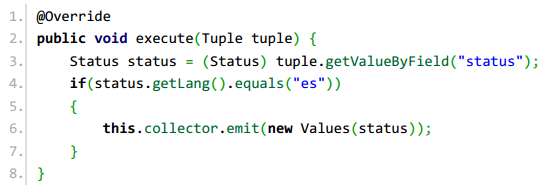
\includegraphics[scale=0.8]{images/LanguageBoltExecute.png}
	\caption[Implementación del método \textit{execute} del \textit{bolt} de idioma.]{Implementación del método \textit{execute} del \textit{bolt} de idioma.\\Fuente: Elaboración Propia, (2016)}
	\label{fig:operadorIdioma}
\end{figure}

\subsubsection*{Operador filtro de consultas}
\label{subsubsec:2op}

El segundo nivel de operadores consiste en un segundo filtro, en este caso, los filtros introducidos por el usuario para discriminar \textit{tweets} según su contenido. Esto busca centrar la atención del sistema en los términos importantes para el usuario. De esta forma la cantidad de datos que ingresa al sistema puede verse reducida aún más en función de qué términos se hayan sido especificados.

Adicionalmente a lo anterior se encuentra que la historia HU-c02. Esta historia menciona la necesidad de incrementar los términos de búsqueda para enriquecerla y así incrementar la cantidad de \textit{tweets} relacionados al evento. Para realizar esto se consideró una práctica del procesamiento de lenguaje natural como es la denominada \textit{Query Expansion} (QE). Según lo descrito por \cite{IRQE} son técnicas comunes al utilizar QE la búsqueda de sinónimos (uso de diccionarios priviamente establecidos), diccionarios basados en la minería de los elementos previamente hayados, creación de diccionadios basados en la co-ocurrencia de términos, es decir, términos que suelen venir juntos o un vocabulario mantenido por editores humanos. Para este trabajo sólo se consideran las dos primeras: Búsqueda por diccionario de sinónimos y una implementación que encuentra los términos más frecuentes dentro de los resultados de la búsqueda.

El diccionario de sinónimos corrresponde básicamente una bolsa de palabras asociadas a una semilla, es decir, dado un término de búsqueda, se agregan tantos términos nuevos a este filtro como sinónimos estén relacionados a al término en cuestión.

Para el caso de la búsqueda de términos frecuentes mencionada anteriormente, se sugirió integrar un proyecto \textit{Storm} ya desarrollado el cuál tiene por finalidad la búsqueda de los denominados \textit{trending topics}, es decir, aquellos términos de los que se realizan más menciones en un determinado instante, pero aquella implementación sólo consideraba los denominados \textit{hashtag}, un marcador de palabras concatenadas que inician por el caracter ``\#". Siendo ese el caso el uso de esta topología \textit{Storm} no es del todo útil. En su lugar se desarrolla un contador de frecuencias para palabras con un funcionamiento similar, dicha implementación se aprecia en el Algoritmo \ref{alg:TT}.\\

\begin{algorithm}[H]\setstretch{1.5}
	\begin{algorithmic}[numeracion_lineas]
		\REQUIRE Estados $E=\{e_{1}, \dots, e_{n} \}$.
		\ENSURE Terminos frecuentados $T=\{t_{1}, \dots, t_{10} \}$.
		\STATE Lista de terminos: $l$.
		\FOR{Estado: $e_{i}$}
			\STATE Dividir estado por palabra.
			\STATE Eliminar \textit{stopword} de las palabras.
			\FOR{Palabra: $w_{i}$ en $e_{i}$}
				\IF{ $w_{i}$ está en  $l_{i}$}
					\STATE aumentar contador de $w_{i}$ en $l_{i}$.
				\ELSE
					\STATE agregar $w_{i}$ a $l_{i}$ con contador en 1.
				\ENDIF		
			\ENDFOR
		\ENDFOR
		\IF{$l_{i}$ tiene menos de 10 elementos}
			\RETURN $l_{i}$
		\ELSE
			\RETURN los 10 primeros elementos de $l_{i}$.
		\ENDIF
	\end{algorithmic}
	\caption{Algoritmos de términos recurrentes.}
	\label{alg:TT}
\end{algorithm}\vphantom\\

Dado que el operador puede estar replicado no se reciben los mismos \textit{tweets} en todas sus instancias, por ello este proceso se realiza de manera única para cada instancia en función de los estados que hayan llegado a él. El Algoritmo \ref{alg:TT} agrega a los términos de búsqueda de cada instancia las palabras más frecuentes y, siguiendo el ejemplo de \textit{Twitter} con sus \textit{trending topics}, tiene un máximo de diez nuevos términos de búsqueda.

\begin{figure}[H]
	\centering
	\captionsetup{justification=centering}
	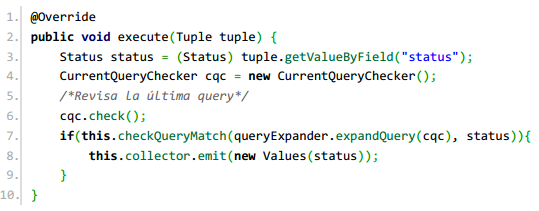
\includegraphics[scale=0.8]{images/FilterBolt.png}
	\caption[Implementación del método \textit{execute} del \textit{bolt} del filtro de consultas.]{Implementación del método \textit{execute} del \textit{bolt} del filtro de consultas.\\Fuente: Elaboración Propia, (2016)}
	\label{fig:operadorFiltro}
\end{figure}

La Figura \ref{fig:operadorFiltro} muestra la implementación del filtro de consultas. El filtro de consultas hace uso de instancias de los objetos descritos en HU-v05 para encontrar la última consulta en el sistema y expande la consulta según ésta y los resultados obtenidos en los estados recibidos. Finalmente, si el \textit{tweet} contiene algunos de los términos especificados, se emite al siguiente nivel de operadores.

\subsubsection*{Operador normalizador de texto}
\label{subsubsec:3op}

El tercer problema es inherente a \textit{Twitter}: En esta red social es común referenciar un estado a un determinado tema, he ahí el uso de los conocidos \textit{Hashtag} que, como se mencionó en la sección \ref{subsubsec:estadisticasdeproc} corresponden a palabras concatenadas antecedidas por el caracter \#. Otro problema común corresponde a la mención de usuarios, la cual se trata de una referencia al nombre de usuario dentro de la aplicación antecedida por el caracter ``@" (usualmente utilizada para el envío de mensajes entre pares). Diversos autores, entre ellos, \cite{NLPaccuracy}, \cite{NLPaccuracy1} y \cite{NLPaccuracy2}, han señalado que la existencia de estos elementos significan una disminución en la precisión de los elementos descritos en la sección \ref{sec:diseno:clasificador}. Dado lo anteriormente expuesto, él tercer operador corresponde a normalizador de texto, el cual reemplaza menciones a usuarios, \textit{hashtags} y URLs, todas ellas de contenido variable, por palabras marcadoras. El reemplazo a realizarse se muestra en la Tabla \ref{tab:reemplazosDeEntidades}.

\begin{table}[H]
\centering
\caption[Reemplazo de entidades en texto.]{Reemplazo de entidades en texto.\\Fuente: Elaboración Propia, (2016)}
\label{tab:reemplazosDeEntidades}
\begin{tabular}{|c|c|}
\hline
\textbf{Entidad} & \textbf{Marcador} \\ \hline
@usuario         & USUARIO            \\ \hline
\#hashtag        & HASHTAG            \\ \hline
http://var.foo/  & URL                \\ \hline
\end{tabular}
\end{table}

La implementación de este operador se realizó utilizando expresiones regulares para detectar cuándo se está haciendo referencia a uno de los elementos anteriores y luego aplicar su reemplazo.

\subsubsection*{Operador geolocalizador}
\label{subsubsec:4op}

El cuarto operador presentado tiene relación, principalmente, con la historia HU-v01. Si bien se mencionó cómo se realiza la visualización, no se señaló cómo es que se obtienen tanto la coordenadas geográficas, latitud y longitud, para ubicar geográficamente un evento.

Se ha señalado por \cite{ChatoSurvey} que menos del 1\% de los \textit{tweets} contienen datos en sus campos correspondientes a geolocalización. En un experimento (véase Apéndice \ref{apendice:apendice1}) realizado utilizando la herramienta \textit{RapidMiner} se obtuvo una muestra de 67.789 \textit{tweets} directamente desde el \textit{stream} sin utilizar filtros de búsqueda, de esos \textit{tweets} 67.475 no contaban con los datos correspondientes a la ubicación geográfica, es decir, el 0.46\% de los datos de aquella muestra cuentan con la información requerida, lo que hace creer que lo presentado por los autores antes mencionados, está en lo correcto.

Siendo la geolocalización un elemento de suma importancia para el funcionamiento de la aplicación, es necesario construir un mecanismo alternativo capaz de asociar los eventos a lugares geográficos. Para llevar a cabo esta tarea, se propone explotar el contenido del \textit{tweet} para buscar lugares geograficos explícitamente mencionados en el texto. Para ello se generó de manera manual un diccionario con todas las comunas del país y sus coordenadas geograficas y se diseñó el Algoritmo \ref{alg:geolocalizacion}. De esta manera existe una aproximación para detectar la ubicación a la que un \textit{tweet} hace referencia.\\

\begin{algorithm}[H]\setstretch{1.5}
	\begin{algorithmic}[numeracion_lineas]
		\REQUIRE Lista de ciudades $C=\{c_{1}, \dots, c_{n} \}$.
		\REQUIRE Tweet $t$.
		\ENSURE Coordenadas geográficas $P=\{latitud, longitud\}$.
		\IF{$t$ está geolocalizado}
			\IF{Está dentro del territorio chileno}
				\RETURN Coordenadas del $t$.
			\ELSE
				\RETURN Fuera de Chile.
			\ENDIF
		\ELSE
			\IF{El texto de $t$ contiene elementos presentes en $C$}
				\RETURN Coordenadas de $c_{i}$.
			\ELSE
				\RETURN No geolocalizable.
			\ENDIF
		\ENDIF
	\end{algorithmic}
	\caption{Algoritmos de ubicación geoográfica.}
	\label{alg:geolocalizacion}
\end{algorithm}\vphantom\\

Haciendo uso del algoritmo desarrollado es posible aumentar la cantidad de elementos que continúan siendo procesados por el sistema, en lugar de utilizar sólo el porcentaje de datos que contienen datos de la ubicación, pero se ha de recalcar que un dato cuya ubicación no pueda ser obtenida no continuará al siguiente nivel de operadores de la topología. Su efectividad radica en la aparición del nombre de una localidad chilena en el texto.

\subsubsection*{Operador removedor de \textit{stopword}}
\label{subsubsec:5op}

Existen palabras que, según lo descrito en \cite{IRQE} y presentado por \cite{JustifStopStemm}, aportan poco o nada información al texto, estas palabras son denominadas \textit{stopwords} y se componen de artículos, pronombres, preposiciones, etcétera. Este operador hace uso de una lista de \textit{stopwords}, las que son son eliminadas del texto que se está procesando, para ello se hace uso del Algoritmo \ref{alg:stopwords} presentado a continuación.\\

\begin{algorithm}[H]\setstretch{1.5}
	\begin{algorithmic}[numeracion_lineas]
		\REQUIRE Lista de \textit{stopwords} $S=\{s_{1}, \dots, s_{n} \}$.
		\REQUIRE Texto $T$.
		\ENSURE Texto $T'$.
		\STATE $T'$ = $T$
		\FOR{cada palabra de $T$, $t_{i}$}
			\IF{$t_{i}$ está contenida en $S$}
			\STATE $T'$ = $T'$ - $t_{i}$. 
			\ENDIF
		\ENDFOR
		\RETURN $T'$
	\end{algorithmic}
	\caption{Algoritmos de eliminiación de \textit{stopwords}.}
	\label{alg:stopwords}
\end{algorithm}\vphantom\\

\subsubsection*{Operador raíz de texto}
\label{subsubsec:6op}

Un clasificador no sabe reconocer que palabras, por ejemplo, en diferente tiempo verbal hacen referencia a lo mismo y las procesa como dos elementos independientes, para evitar aquello una técnica común en el procesamiento de lenguaje natural, más específicamente en la clasificación de texto, es llevar las palabras a una raíz común para ahorrar este problema al clasificador.

Este operador hace uso del algoritmo de \cite{Porter}, para extraer prefijos y sufijos de palabras y llevarlas a una raíz común, \cite{StemmingLema}, son ejemplos de este proceso, denominado \textit{stemming}, las palabras presentadas en la Tabla \ref{tab:ejstemming}

\begin{table}[H]
\centering
\caption[Ejemplo de \textit{stemming} para la palabra ``presentar".]{Ejemplo de \textit{stemming} para la palabra ``presentar"'.\\Fuente: Elaboración Propia, (2016)}
\label{tab:ejstemming}
\begin{tabular}{|c|c|}
\hline
\textbf{Palabra} & \textbf{Combinaciones de Sufijos} \\ \hline
Presentarla      & arla                              \\ \hline
Presentarlas     & arlas                             \\ \hline
Presentarle      & arle                              \\ \hline
Presentarles     & arles                             \\ \hline
Presentarlo      & arlo                              \\ \hline
Presentarlos     & arlos                             \\ \hline
Presentarse      & arse                              \\ \hline
Presentase       & ase                               \\ \hline
Presentásemos    & ásemos                            \\ \hline
Presente         & e                                 \\ \hline
Presentémonos    & émonos                            \\ \hline
\end{tabular}
\end{table}

\subsubsection*{Operador etiquetador}
\label{subsubsec:7op}

El funcionamiento principal del sistema está en detectar necesidades expresadas en el texto. Para ello se construyó un clasificador bayesiano (cuyo detalle de construcción se presenta en las más adelante en esta sección). En primer lugar, se recibe desde los operadores previos, un texto preparado para ser etiquetado, este texto es transformado en \textit{tokens} (un vector de elementos donde cada elemento corresponde a una palabra) y posteriormente es entregado a Mallet, herramienta que hace uso del clasificador construido y, según el resultado de la evaluación, le asigna la correspondiente etiqueta. 

Al contar con este dato ya se está en condiciones de generar un nuevo marcador, pues se tienen todos los elementos necesarios en un documento de la colección marcadores presentados en la Figura \ref{fig:esquemaMarker2}, así entonces los datos recibidos más la etiqueta correspondiente a la clasificación son emitidas para ser recibidas por el operador de persistencia.

\subsubsection*{Operador persistencia}
\label{subsubsec:8op}

Habiendo pasado por todos los operadores descritos anteriormente es necesario comunicar los nuevos eventos detectados al visualizador para que los posicione en el mapa. Para ello se hace uso de la base de datos, como fue explicado en la sección \ref{sec:diseno:comunicacion}.
Este operador se encarga de conectarse a la base de datos y almacenar el nuevo marcador. Los datos recibidos desde la cadena de procesamiento se llevan a una instancia de objeto Java, llamado ``Marker", el cual contiene los mismos elementos descritos para un documento de la colección ``Markers", a un objeto JSON utilizando \textit{Jongo} que lo transforma en BSON para almacenarlo en la base de datos en MongoDB.

\subsubsection*{Proceso de construcción del clasificador}
\label{subsubsec:clasificacion}

Hasta ahora se han tocado, prácticamente, todos los temas que se relacionan con el funcionamiento del sistema de detección, desde donde se obtienen los datos, por que operadores pasa para ser procesado e incluso como se almacenan, pero no se ha especificado cómo se realiza la clasificación, es decir, cómo dado un texto de entrada se consigue discriminar en qué categoría encaja. Esta sección busca dar a conocer el proceso de construcción del clasificador haciendo uso de la metodología KDD.
	
El concepto que involucra la construcción de un clasificador es el de ``aprendizaje supervizado", que fue mencionado en la sección \ref{subsec:MineriaTexto}. En este tipo de aprendizaje se requiere de un conjunto de datos de entrada, denominados conjunto de entrenamiento, que ha de pasar por el algoritmo, en este caso \textit{Naïve Bayes}, que ha de conocer previamente la salida esperada para cada elemento del conjunto. El resultado esperado es un clasificador capaz de predecir, en este caso, a qué categoría pertenece un texto sometido a su evaluación.

Según la metodología KDD existen subprocesos en la búsqueda de conocimiento en bases de datos, estos fueron descritos en la sección \ref{subsec:MetodologiaDetalle}, para este caso particular se describe cómo fue realizado cada uno de estos subprocesos para la construcción del clasificador con el que cuenta el sistema.

El subproceso de selección de datos se llevó a cabo extrayendo un subconjunto del \textit{dataset} mencionado en la sección \ref{subsec:alcances}. Este conjunto, de exactamente 2234 \textit{tweets} correspondientes al terremoto de Concepción el año 2010, todos ellos en español, pero no todos referencian al evento, pues coincidió con la realización de la LI versión del Festival Internacional de la Canción de Viña del Mar y muchos de estos \textit{tweets} hacen referencian a este último. Los datos en este punto de proceso cuentan con los campos correspondientes a un \textit{tweet} de la época, es decir: ``ID\_unit", ``day", ``date", ``time\_zone", ``time", ``tweet\_it", ``user\_id", ``name", ``screen\_name", ``friends\_count", ``follower\_count", ``text" y ``value". Todos ellos separados por coma (,).

En cuanto al subproceso de preprocesamiento de datos, el primer paso corresponde a la limpieza de los datos, el conjunto de datos que se utilizó contenía elementos incompletos que no presentaban texto, estos fueron eliminados, pues no resultaban útiles sin este componente, quedando así un total de 2187 \textit{tweets} con datos útiles.

El siguiente paso corresponde al suproceso de transformación de datos. Del conjunto de datos útiles se extrajo el texto y se eliminaron todos los demás componentes. Llegados a este punto sólo se contaba con una lista de textos de \textit{tweets} en español. Lo siguiente a realizar corresponde al proceso de etiquetado, para ello se leyó cada una de las entradas de texto y según su contenido se ubicó manualmente en alguna de las categorías descritas en la sección \ref{sec:diseno:categorias}. Además se asignó un identificador a cada texto basado en su posición en la lista, para ser ingresados a la herramienta Mallet, encargada de la construcción del clasificador. Así se obtuvo un archivo con los datos formateados según lo descrito en la sección \ref{sec:diseno:clasificador}, es decir, con los campos ``Identificador", ``Etiqueta", ``Contenido". En este punto los datos fueron ingresados al sistema para la aplicación de los operadores descritos en la sección \ref{subsec:detectorNecesidades}, en particular la eliminación de \textit{stopwords}, normalización de texto y \textit{stemming}.

El cuarto subproceso es automatizado por Mallet y corresponde al minado de texto en sí. Para entregarle los datos a Mallet primero han de construirse como un objeto ``\textit{Instance}", lo cual se realiza entregándole cada uno de los elementos preparados en la sección anterior: el identificador, etiqueta y contenido que ya ha pasado por las operaciones que componen el subproceso de transformación. Se configuró Mallet para construir un clasificador utilizando un 90\% del conjunto para entrenar y un 10\% para realizar la evaluación. Como resultado de este proceso se obtiene un objeto \textit{Classifier}, el cual puede ser serializado y almacenado como un archivo denominado, en este caso, ``classifier.dene". 

Finalmente, el subproceso de evaluación también es llevado a cabo por la herramienta Mallet, que implementa un objeto denominado ``\textit{Trial}" el cual, utilizando el clasificador y un conjunto de datos de prueba realiza la evaluación de este. Como resultado de este subproceso se obtienen las métricas comunes de evaluación: \textit{accuracy}, \textit{recall} y \textit{F-1 score}. La evaluación del clasificador construido se presenta en la sección \ref{sec:EvalClassificador} del Capítulo \ref{sec:EvalClassificador}. 

\subsubsection*{Topología del sistema}
\label{subsubsec:topologiaSistema}

Habiendo definido los elementos de procesamiento, los operadores o \textit{Bolts}, se pasa definir la topología. La topología que utiliza el sistema está definida en la Figura \ref{fig:TopologiaGeneral}.

La razón de este orden en la topología se debe a varias razones y se justifican a continuación:

\begin{itemize}
\item \textit{Spout Twitter}: es el eslabón principal de la cadena. Desde aquí se emiten los nuevos estados al sistema y todo el sistema depende de él. 
\item \textit{Bolt} Filtro de idioma: ocupa la primera posición de los operadores del sistema, dado que se espera que el \textit{stream} reciba estados de todo el mundo y no sólo en español. Al estar este operador en primer lugar se reduce el flujo en gran medida, lo cual puede comprobarse por los resultados obtenidos en el Capítulo \ref{cap:experimentos}.
\item \textit{Bolt} Filtro de consulta: habiendo filtrado sólo aquellos estados cuyo lenguaje sea el español, es necesario filtrar aun más el \textit{stream} valiéndose de las restricciones especificadas por el usuario. Así sólo los estados que contengan términos especificados por el usuario, o el sistema de expansión, continúan en el sistema.
\item\textit{Bolt} Normalizador de texto: Previo al detector de ubicación para evitar posibles confusiones que pueda acarrear la existencia de nombres de lugares en elementos como nombres de usuario, \textit{hashtags} o enlaces.
\item\textit{Bolt} Detección de ubicación: Ocupa esta posición, pues debe ir previo a la eliminación de \textit{stopwords}, de lo contrario ubicaciones, como por ejemplo ``Los Vilos", válida dentro de Chile, es ignorada por el sistema.
\item\textit{Bolt} Eliminador de \textit{stopword}: Se realiza previo al \textit{stemming} para reducir la carga computacional, pues el operador de \textit{stemming} lleva a palabras raíz estos términos que no son necesarios.
\item\textit{Bolt} \textit{Stemmer}: Es la única ubicación posible para este operador, pues el siguiente paso es etiquetar el estado.
\item\textit{Bolt} Etiquetador: Aplica el modelo al estado, el estado ha de tener su correspondiente etiqueta antes de ser almacenado.
\item\textit{Bolt} Persistencia: último eslabón de la cadena. Ingresa un nuevo documento a la colección de marcadores.
\end{itemize}

\begin{figure}[H]
	\centering
	\captionsetup{justification=centering}
	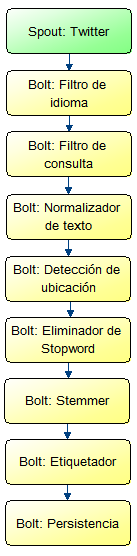
\includegraphics[scale=0.8]{images/TopologiaGeneral.png}
	\caption[Topología general del sistema.]{Topología general del sistema.\\Fuente: Elaboración Propia, (2016)}
	\label{fig:TopologiaGeneral}
\end{figure}

Puede verse que corresponde a una topología lineal, cada operador estará replicado dependiendo de su carga y con un máximo definido por el administrador del sistema. Existe la posibilidad de hacer uso de algoritmos automáticos para ajustar el nivel de replicación, sin embargo está fuera de los alcances del proyecto.




